%%% Article: Software System for Data Acquisition and Analysis Operating the ATLAS-TPX Network
%%% Authors: Petr Manek, Jakub Begera
%%% Copyright (c) 2017 IEAP CTU


\section{\label{sec:hardware}Hardware Architecture}
Given the harsh radiation environment within the ATLAS machine, ATLAS-TPX devices have to be connected to the rest of the system through a dedicated readout interface. This readout is a special hardware device that reads data and controls acquisition of the detector. The ATLASPIX readout (see Fig.~\ref{fig:device_with_readout}) was developed by modifying a regular FITPix readout~\cite{FITPix}.

\begin{figure}[tbp]
	\centering
  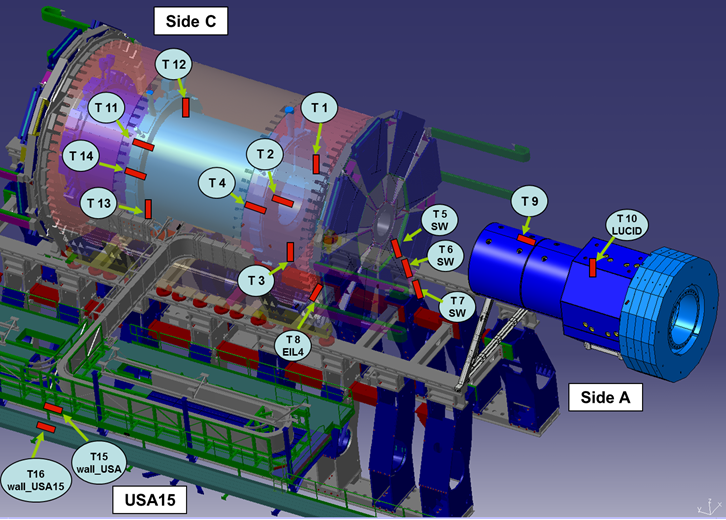
\includegraphics[clip, width=.45\textwidth, angle=0]{Plots/ATLASTPX.png}
  \caption {Artistic view of the device positions of the ATLAS-TPX network in the ATLAS experiment.}
  \label{fig:positions}
\end{figure}

The readout has two parts connected by four cables. The detector itself is positioned and oriented within the ATLAS machine (see Fig.~\ref{fig:positions}), whereas the rest of the readout is placed in a nearby server room, shielded against ionizing radiation. Cables connect both parts, allowing protected hardware to control detectors remotely during operation of the machine. To manage multiple detectors simultaneously, a computer is directly connected to all readouts. This \textit{Control PC} gathers all measured data and forwards commands from the system operator to the detectors through the ATLASPIX readout.

\begin{figure}[tbp]
	\centering
  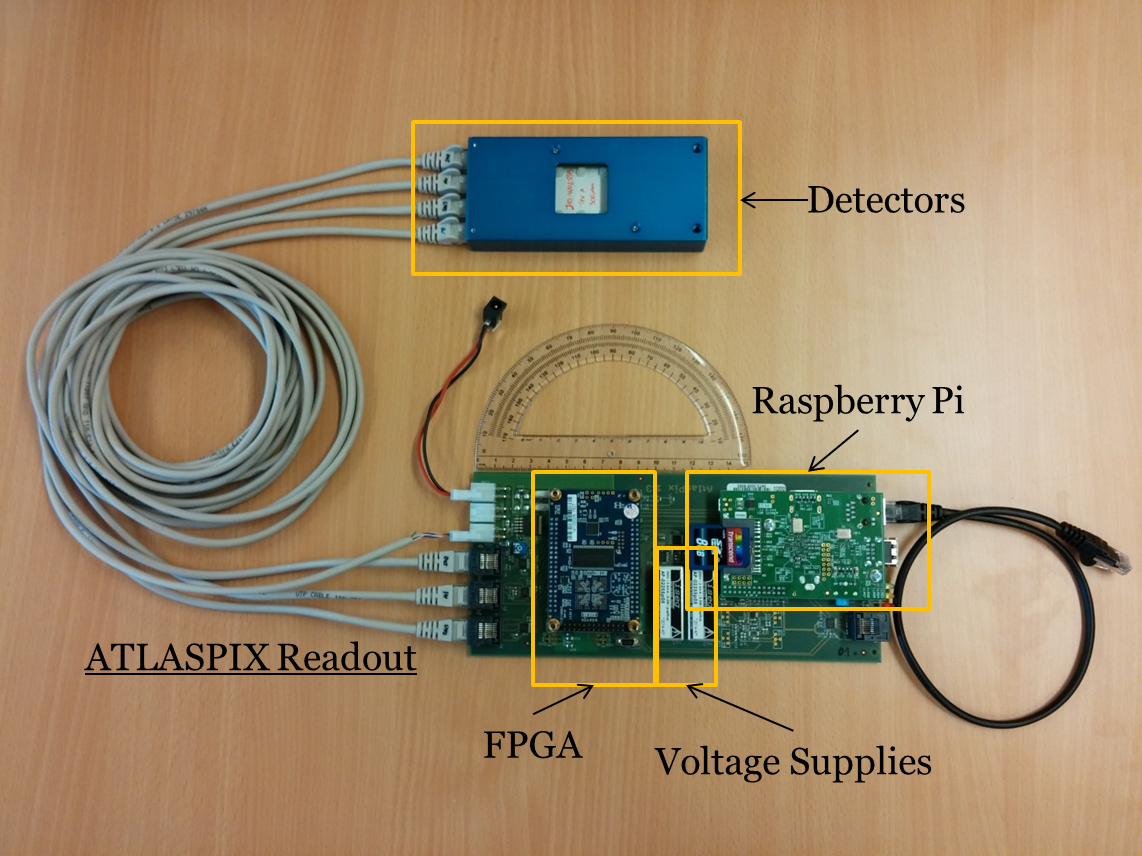
\includegraphics[clip, width=.45\textwidth, angle=0]{Plots/ATLASPIX.png}
  \caption {ATLAS-TPX device, connected to its readout system through three Ethernet cables. The readout system consists of an FPGA, handling the device settings and operation, and a Raspberry Pi minicomputer for sending the data to the control PC in human readable format. Two voltage supplies are used for feeding the proper bias to each of the sensor layers.}
  \label{fig:device_with_readout}
\end{figure}

The Control PC (seen in Fig.~\ref{fig:rack}) is connected directly to the ATLAS Technical Network, which is isolated from the rest of CERN network infrastructure. Consequently, all communications outside the network have to utilize other systems. Acquisition control and real-time status monitoring of the network uses DCS (Detector Control System). Measured data are transferred to the EOS distributed storage system~\cite{MAscetti2015,Peters2011}.

\begin{figure}[tbp]
	\centering
  \includegraphics[clip, width=.33\textwidth, angle=0]{Plots/rack_usa15.pdf}
  \caption {TPX rack in the shielded technical room USA15 in the ATLAS cavern. The photo shows the installed ATLASPIX readouts connected to the Control PC, which communicates with DCS, EOS and FSM over the ATLAS Technical Network.}
  \label{fig:rack}
\end{figure}
